\chapter{目标跟踪}

目标跟踪(Target Tracking)是雷达信号处理与信息融合中的核心任务,其目标是在连续时间序列的量测数据中,对运动目标的状态进行实时估计与更新,并在存在多目标和杂波干扰的情况下实现可靠的航迹维持。通常而言,目标跟踪面临两个基本问题:其一是状态估计,即在噪声环境下对目标的动力学状态(位置、速度、加速度等隐含量)进行递推估计;其二是数据关联,即在多目标与虚警并存的量测环境中,判断每个观测量应当归属于哪一条目标航迹。本章将围绕这两个关键问题展开,首先介绍状态估计方法,然后讨论数据关联方法,以此构建目标跟踪的基本理论框架。

\section{状态估计}
在前述目标检测与参数估计的基础上,可以获得目标的多种观测信息,如距离、方位与速度等。然而在实际应用中,这些观测量不可避免地受到噪声与干扰的影响,因而存在偏差与不确定性。为了提升信息的可靠性,需要综合利用历史量测进行处理,实现对观测序列的降噪与平滑,并进一步完成对目标未来状态的预测。这便构成了状态估计问题的核心任务,也是实现高精度目标跟踪的前提。

\subsection{最小均方滤波}

不妨假设在第\( t \)时刻,目标的状态向量为\( \bm{x}_t \in \mathbb{R}^M \),其可包含目标的速度、加速度等多种状态变量。同时,假设在该时刻可以获得一个观测向量\( \bm{z}_t \in \mathbb{R}^N \),其可能是目标的距离、方位等测量值。在线性假设下,观测向量与目标状态向量之间的关系通常可以使用如下模型来描述:
\[
    \bm{z}_t = \mathbf{H} \bm{x}_t + \bm{v}_t,
\]
其中,$\mathbf{H} \in \mathbb{R}^{N \times M}$ 为待估计的观测矩阵,用于刻画状态向量与观测向量之间的线性映射关系;$\bm{v}_t$ 为观测噪声,通常假设其服从零均值高斯分布。最小二乘算法(Least Squares, LS)的目标是在对观测数据进行处理时,最小化估计误差的均方值,从而获得对目标状态的最优估计。若共获得 $T$ 次观测,则相应的优化问题可表述为:
\[
    \min_{\mathbf{H}_T} \ \frac{1}{T}\sum_{t=1}^{T} \big\| \mathbf{H}_T\bm{x}_t - \bm{z}_t \big\|^2,
\]
其中,\( \mathbf{H}_T \) 表示利用前 \( T \) 次观测数据估计得到的观测矩阵。

记
\[
    \mathbf{X}_T = \begin{bmatrix} \bm{x}_1 & \bm{x}_2 & \cdots & \bm{x}_T \end{bmatrix} \in \mathbb{R}^{M \times T},
    \quad
    \mathbf{Z}_T = \begin{bmatrix} \bm{z}_1 & \bm{z}_2 & \cdots & \bm{z}_T \end{bmatrix} \in \mathbb{R}^{N \times T},
\]
则上述优化问题可进一步简化为(方便起见,常数项\( \frac{1}{T} \) 被省略)
\[
    \min_{\mathbf{H}} \big\| \mathbf{H}_T \mathbf{X}_T - \mathbf{Z}_T \big\|_{\mathrm{F}}^2.
\]
利用克罗内克积的相关性质(\cref{cor:kronecker-vec}), \( \mathbf{H}_T \mathbf{X}_T \)可以改写为如下的矩阵乘向量的形式:
\[
    \operatorname{vec}(\mathbf{H}_T \mathbf{X}_T) = \operatorname{vec}(\mathbf{I} \mathbf{H}_T \mathbf{X}_T)  = (\mathbf{X}_T^{\mathrm{T}} \otimes \mathbf{I}) \operatorname{vec}(\mathbf{H}_T),
\]
其中,\( \mathbf{I} \in \mathbb{R}^{N \times N} \) 为单位矩阵。于是,优化问题可转化为
\[
    \min_{\operatorname{vec}(\mathbf{H}_T)} \left\| (\mathbf{X}_T^{\mathrm{T}} \otimes \mathbf{I}) \operatorname{vec}(\mathbf{H}_T) - \operatorname{vec}(\mathbf{Z}_T) \right\|^2.
\]
该问题为标准的线性最小二乘问题,其解析解为
\[
    \begin{split}
        \operatorname{vec}(\mathbf{H}_T) & = \left( (\mathbf{X}_T^{\mathrm{T}} \otimes \mathbf{I})^{\mathrm{T}} (\mathbf{X}_T^{\mathrm{T}} \otimes \mathbf{I}) \right)^{-1} (\mathbf{X}_T^{\mathrm{T}} \otimes \mathbf{I})^{\mathrm{T}} \operatorname{vec}(\mathbf{Z}_T ) \\
                                         & = \left( \left( \mathbf{X}_T \mathbf{X}_T^{\mathrm{T}} \right)\otimes \mathbf{I} \right)^{-1} (\mathbf{X}_T \otimes \mathbf{I}) \operatorname{vec}(\mathbf{Z}_T)                                                               \\
                                         & = \left( \left( \mathbf{X}_T \mathbf{X}_T^{\mathrm{T}} \right)^{-1} \otimes \mathbf{I} \right) (\mathbf{X}_T \otimes \mathbf{I}) \operatorname{vec}(\mathbf{Z}_T)                                                              \\
                                         & = \left( \left( \mathbf{X}_T \mathbf{X}_T^{\mathrm{T}} \right)^{-1} \mathbf{X}_T \otimes \mathbf{I} \right) \operatorname{vec}(\mathbf{Z}_T)                                                                                   \\
    \end{split}
\]
再次利用\cref{cor:kronecker-vec},可得
\[
    \mathbf{H}_T = \mathbf{Z}_T \mathbf{X}_T^{\mathrm{T}} \left( \mathbf{X}_T \mathbf{X}_T^{\mathrm{T}} \right)^{-1}.
\]

注意到,随着观测次数 \(T\) 的增加,观测矩阵 \(\mathbf{X}_T\) 的规模不断增大,从而导致计算复杂度迅速提升。另一方面,目标的运动状态也可能随时间发生变化,因此没有必要始终依赖全部历史观测数据来估计观测矩阵 \(\mathbf{H}_T\)。基于此,可以考虑采用递推方式对观测矩阵进行逐步更新。假设在时刻 \(T\) 已经得到了估计矩阵 \(\mathbf{H}_{T}\),当引入第 \(T+1\) 次观测后,仅利用该次观测来修正已有估计。相应的优化问题为
\[
    \min_{\mathbf{H}_{T}} \ \big\| \mathbf{H}_{T} \bm{x}_{T+1} - \bm{z}_{T+1} \big\|^2.
\]
该目标函数关于 \(\mathbf{H}_{T}\) 的梯度为
\[
    \nabla_{\mathbf{H}_{T}} = 2\big(\mathbf{H}_{T} \bm{x}_{T+1} - \bm{z}_{T+1}\big)\bm{x}_{T+1}^{\mathrm{T}}.
\]
其中,\(\mathbf{H}_{T}\bm{x}_{T+1}-\bm{z}_{T+1}\) 即为利用当前估计矩阵对最新观测进行预测时所产生的误差。记作
\[
    \bm{e}_{T+1} = \mathbf{H}_{T}\bm{x}_{T+1} - \bm{z}_{T+1},
\]
则可采用梯度下降法更新观测矩阵:
\[
    \mathbf{H}_{T+1} = \mathbf{H}_{T} + \mu\, \bm{e}_{T+1}\bm{x}_{T+1}^{\mathrm{T}},
\]
其中 \(\mu > 0\) 为步长参数。这种利用随机梯度下降(Stochastic Gradient Descent, SGD)的进行更新方法被称为最小均方(Least Mean Square, LMS)算法。可以发现其核心思想在于:每次引入新观测时,先利用当前观测矩阵进行预测并计算预测误差,随后结合该误差与当前观测对观测矩阵进行修正,从而实现动态更新。

在实际应用中,步长参数 \(\mu\) 的选取对算法的收敛性与稳定性具有重要影响。若 \(\mu\) 过大,可能导致算法发散;若 \(\mu\) 过小,则收敛速度较慢。而递推最小均方(Recursive Least Mean Square, RLMS)算法,一方面通过引入遗忘因子\( \lambda \in (0,1] \)来减小对早期观测数据的依赖,另一方面通过巧妙地利用伍德伯里矩阵恒等式(Woodbury Matrix Identity, 见\cref{cor:woodbury-matrix-identity})来高效地更新估计矩阵,无需选取步长参数,从而提升了算法的性能与鲁棒性。具体而言,在时刻 \( T \) 时,优化问题可表述为
\[
    \min_{\mathbf{H}_T} \ \sum_{t=1}^{T} \lambda^{T-t} \big\| \mathbf{H}_T\bm{x}_t - \bm{z}_t \big\|^2.
\]

同样可以将上述问题转化为矩阵形式:
\[
    \min_{\mathbf{H}_T} \ \big\| \mathbf{H}_T \mathbf{X}_T - \mathbf{Z}_T\big\|_{\mathrm{F}}^2,
\]
其中,
\[
    \mathbf{X}_T = \begin{bmatrix} \sqrt{\lambda}^{T-1}\bm{x}_1 & \sqrt{\lambda}^{T-2}\bm{x}_2 & \cdots & \bm{x}_T \end{bmatrix} \in \mathbb{R}^{M \times T},
\]
\[
    \mathbf{Z}_T = \begin{bmatrix} \sqrt{\lambda}^{T-1}\bm{z}_1 & \sqrt{\lambda}^{T-2}\bm{z}_2 & \cdots & \bm{z}_T \end{bmatrix} \in \mathbb{R}^{N \times T}.
\]
与普通最小二乘相同,\( T \)时刻该问题的解析解为
\[
    \mathbf{H}_T = \mathbf{Z}_T \mathbf{X}_T^{\mathrm{T}} \left( \mathbf{X}_T \mathbf{X}_T ^{\mathrm{T}} \right)^{-1},
\]
而\( T + 1 \)时刻的解为
\[
    \mathbf{H}_{T+1} = \mathbf{Z}_{T+1} \mathbf{X}_{T+1}^{\mathrm{T}} \left( \mathbf{X}_{T+1} \mathbf{X}_{T+1} ^{\mathrm{T}} \right)^{-1}.
\]

注意到,矩阵\( \mathbf{X}_T \)和\( \mathbf{X}_{T+1} \)之间,矩阵\( \mathbf{Z}_T \)和\( \mathbf{Z}_{T+1} \)之间, 存在如下关系:
\[
    \mathbf{X}_{T+1} = \begin{bmatrix} \sqrt{\lambda} \mathbf{X}_T & \bm{x}_{T+1} \end{bmatrix}, \quad  \mathbf{Z}_{T+1} = \begin{bmatrix} \sqrt{\lambda} \mathbf{Z}_T & \bm{z}_{T+1} \end{bmatrix}.
\]
因此,\( \mathbf{Z}_{T+1} \mathbf{X}_{T+1}^\mathrm{T} \)可以写成如下的形式:
\[
    \mathbf{Z}_{T+1} \mathbf{X}_{T+1}^\mathrm{T} = \begin{bmatrix} \sqrt{\lambda} \mathbf{Z}_T & \bm{z}_{T+1} \end{bmatrix} \begin{bmatrix}
        \sqrt{\lambda} \mathbf{X}_T^\mathrm{T} \\
        \bm{x}_{T+1}^\mathrm{T}
    \end{bmatrix} = \lambda \mathbf{Z}_T \mathbf{X}_T^\mathrm{T} + \bm{z}_{T+1}\bm{x}_{T+1}^\mathrm{T}.
\]
类似地,\( \mathbf{X}_{T+1}  \mathbf{X}_{T+1}^\mathrm{T} \)可以写成如下的形式:
\[
    \mathbf{X}_{T+1}  \mathbf{X}_{T+1}^\mathrm{T} = \begin{bmatrix} \sqrt{\lambda} \mathbf{X}_T & \bm{x}_{T+1} \end{bmatrix} \begin{bmatrix}
        \sqrt{\lambda} \mathbf{X}_T^\mathrm{T} \\
        \bm{x}_{T+1}^\mathrm{T}
    \end{bmatrix} = \lambda \mathbf{X}_T \mathbf{X}_T^\mathrm{T} + \bm{x}_{T+1}\bm{x}_{T+1}^\mathrm{T}.
\]
方便起见,记\( \mathbf{X}_T \mathbf{X}_T^\mathrm{T} = \mathbf{\Sigma}_T \),\( \mathbf{Z}_T \mathbf{X}_T^{\mathrm{T}} = \mathbf{\Gamma}_T \),则进一步利用伍德伯里矩阵恒等式(\cref{cor:woodbury-matrix-identity}),可得
\[
    \begin{split}
        \left( \mathbf{\Sigma}_{T+1} \right)^{-1} & = \left( \lambda \mathbf{\Sigma}_T + \bm{x}_{T+1}\bm{x}_{T+1}^\mathrm{T} \right)^{-1}                                                                                                                                        \\
                                                  & = \frac{1}{\lambda} \left( \mathbf{\Sigma}_T^{-1} - \frac{\mathbf{\Sigma}_T^{-1} \bm{x_{T+1} \bm{x}_{T+1}^\mathrm{T} \mathbf{\Sigma}_T^{-1}}}{\lambda + \bm{x}_{T+1}^\mathrm{T} \mathbf{\Sigma}_T^{-1} \bm{x}_{T+1}} \right) \\
                                                  & = \frac{1}{\lambda} \left( \mathbf{\Sigma}_T^{-1} - \mathbf{\Sigma}_{T}^{-1} \bm{x}_{T+1} \bm{w}_T^{\mathrm{T}} \right),                                                                                                     \\
    \end{split}
\]
其中\( \bm{g}_{T+1} \)为增益向量,有如下表达式:
\[
    \bm{g}_{T+1} = \frac{\mathbf{\Sigma}_T^{-1} \bm{x}_{T+1}}{\lambda + \bm{x}_{T+1}^\mathrm{T} \mathbf{\Sigma}_T^{-1} \bm{x}_{T+1}}.
\]
则\( \mathbf{H}_T \)可以表示为
\[
    \mathbf{H}_T = \mathbf{\Gamma}_T \mathbf{\Sigma}_T^{-1},
\]
而\( \mathbf{H}_{T+1} \)可以表示为
\[
    \begin{split}
        \mathbf{H}_{T+1} & = \mathbf{\Gamma}_{T+1} \mathbf{\Sigma}_{T+1}^{-1} = (\lambda \mathbf{\Gamma}_T + \bm{z}_{T+1}\bm{x}_{T+1}^\mathrm{T}) \mathbf{\Sigma}_{T+1}^{-1} \\
                         & = \lambda \mathbf{\Gamma}_T \mathbf{\Sigma}_{T+1}^{-1} + \bm{z}_{T+1}\bm{x}_{T+1}^\mathrm{T} \mathbf{\Sigma}_{T+1}^{-1}                           \\
    \end{split}
\]

注意到
\[
    \lambda \mathbf{\Gamma}_T \mathbf{\Sigma}_{T+1}^{-1} = \mathbf{\Gamma}_T \left(  \mathbf{\Sigma}_T^{-1} -  \mathbf{\Sigma}_{T}^{-1} \bm{x}_{T+1} \bm{g}_T^{\mathrm{T}} \right) = \mathbf{H}_T - \mathbf{H}_T \bm{x}_{T+1} \bm{g}_T^{\mathrm{T}},
\]
而
\[
    \begin{split}
        \mathbf{\Sigma}_{T + 1}^{-1} \bm{x}_{T+1} & = \frac{1}{\lambda} \left(  \mathbf{\Sigma}_T^{-1} \bm{x}_{T+1} - \frac{\mathbf{\Sigma}_{T}^{-1} \bm{x}_{T+1} \bm{x}_{T+1}^\mathrm{T} \mathbf{\Sigma}_{T}^{-1} \bm{x}_{T+1} }{\lambda + \bm{x}_{T+1}^\mathrm{T} \mathbf{\Sigma}_{T}^{-1} \bm{x}_{T+1}} \right) \\
                                                  & = \frac{ \mathbf{\Sigma}_T^{-1} \bm{x}_{T+1}}{\lambda + \bm{x}_{T+1}^\mathrm{T} \mathbf{\Sigma}_{T}^{-1} \bm{x}_{T+1}} = \bm{g}_{T+1},
    \end{split}
\]
因此,\( \mathbf{H}_{T+1} \)可以进一步简化为
\[
    \begin{split}
        \mathbf{H}_{T+1} & = \mathbf{H}_T - \mathbf{H}_T \bm{x}_{T+1} \bm{g}_T^{\mathrm{T}}  + \bm{z}_{T+1} \bm{g}_T^{\mathrm{T}} = \mathbf{H}_T + (\bm{z}_{T+1} - \mathbf{H}_T \bm{x}_{T+1}) \bm{g}_T^{\mathrm{T}} \\
                         & = \mathbf{H}_T + \bm{e}_{T+1} \bm{g}_{T+1}^{\mathrm{T}}.
    \end{split}
\]
综上,递推最小均方(RLMS)算法的更新公式为
\[
    \begin{cases}
        \text{更新增益向量:}  & \bm{g}_{T+1} = \frac{\mathbf{\Sigma}_T^{-1} \bm{x}_{T+1}}{\lambda + \bm{x}_{T+1}^\mathrm{T} \mathbf{\Sigma}_T^{-1} \bm{x}_{T+1}},                   \\
        \text{更新协方差矩阵:} & \mathbf{\Sigma}_{T+1}^{-1} = \frac{1}{\lambda} \left( \mathbf{\Sigma}_T^{-1} - \mathbf{\Sigma}_{T}^{-1} \bm{x}_{T+1} \bm{g}_T^{\mathrm{T}} \right), \\
        \text{计算预测误差:}  & \bm{e}_{T+1} = \mathbf{H}_{T}\bm{x}_{T+1} - \bm{z}_{T+1},                                                                                           \\
        \text{更新观测矩阵:}  & \mathbf{H}_{T+1} = \mathbf{H}_T + \bm{e}_{T+1} \bm{g}_{T+1}^{\mathrm{T}}.                                                                           \\
        \text{进行预测:}    & \hat{\bm{z}}_{T+1} = \mathbf{H}_{T+1} \bm{x}_{T+1}.                                                                                                 \\
    \end{cases}
\]

由此可见,整个递推过程同样可以理解为:在每次引入新观测时,先利用当前观测矩阵进行预测并计算预测误差,随后结合该误差与增益向量对观测矩阵进行修正,从而实现动态更新。当\(  \lambda = 1 \) 时,该递推公式退化为经典的最小二乘算法,再结合最小均方滤波算法的迭代公式,可见三者本质上均遵循``先预测、后修正''的思想,区别仅在于增益向量\( \bm{w}_T \)的取值不同。

\begin{example}
    利用最小二乘(LS)、最小均方(LMS)与递推最小均方(RLMS)算法对目标轨迹进行预测,目标轨迹如\cref{fig_trace_gt}所示。
    \begin{figure}[htb!]
        \centering
        \begin{subfigure}{.3\textwidth}
            \centering
            \begin{tikzpicture}
                \begin{axis}[
                        ticklabel style={font=\small},
                        label style={font=\small},
                        xtick=\empty, ytick=\empty,
                        grid, axis equal image,
                        legend cell align=left,
                        height=4cm,
                        legend style={
                                at={(1,1)},
                                anchor=north east,
                                font=\tiny,
                                draw=none,
                                fill=none
                            }
                    ]
                    \addplot[
                        c1,
                        thick,
                        mark=*,
                        mark size=0.5pt,
                        mark options={c1, fill=c1!60}
                    ] table[x=x, y=y, col sep=comma] {./img/tracking/tracking_2.csv};
                \end{axis}
            \end{tikzpicture}
            \caption{}
            \label{fig_trace_gt_1}
        \end{subfigure}
        \begin{subfigure}{.65\textwidth}
            \centering
            \begin{tikzpicture}
                \begin{axis}[
                        ticklabel style={font=\small},
                        label style={font=\small},
                        xtick=\empty, ytick=\empty,
                        grid, axis equal image,
                        legend cell align=left,
                        width=8cm,
                        legend style={
                                at={(0,1)},
                                anchor=north west,
                                font=\tiny,
                                draw=none,
                                fill=none
                            }
                    ]
                    \addplot[
                        c1,
                        thick,
                        mark=*,
                        mark size=0.5pt,
                        mark options={c1, fill=c1!60}
                    ] table[x=x, y=y, col sep=comma] {./img/tracking/tracking_1.csv};
                \end{axis}
            \end{tikzpicture}
            \caption{}
            \label{fig_trace_gt_2}
        \end{subfigure}
        \caption{目标轨迹示意图}
        \label{fig_trace_gt}
    \end{figure}
\end{example}

\begin{solution}
    设\( t \)时刻目标的坐标为\( \bm{p}_{t} \),则可以将历史坐标作为状态向量,而当前坐标作为观测向量,即
    \[
        \bm{x}_t = \begin{bmatrix} \bm{p}_{t-1} \\ \vdots \\ \bm{p}_{t-k} \end{bmatrix} \in \mathbb{R}^{2k}, \quad \bm{z}_t = \bm{p}_t \in \mathbb{R}^2,
    \]
    其中,\( k \)为使用的历史坐标数。利用前 \( T \) 次观测数据,可以估计出观测矩阵 \( \mathbf{H}_T \),进而对第 \( T + 1 \) 时刻的目标位置进行预测。选取\( k=4 \)时,预测结果如\cref{fig_trace1,fig_trace2}所示。
    \begin{figure}[htb!]
        \centering
        \begin{subfigure}{.32\textwidth}
            \centering
            \begin{tikzpicture}
                \begin{axis}[
                        ticklabel style={font=\small},
                        label style={font=\small},
                        xtick=\empty, ytick=\empty,
                        grid, axis equal image,
                        legend cell align=left,
                        width=5.8cm,
                        legend style={
                                at={(1,1)},
                                anchor=north east,
                                font=\tiny,
                                draw=none,
                                fill=none
                            }
                    ]
                    \addplot[
                        c1,
                        thick,
                        mark=*,
                        mark size=0.5pt,
                        mark options={c1, fill=c1!60}
                    ] table[x=x, y=y, col sep=comma] {./img/tracking/tracking_2.csv};
                    \addlegendentry{真实轨迹}
                    \addplot[
                        c2,
                        thick,
                        mark=*,
                        mark size=0.5pt,
                        mark options={c2, fill=c2!60}
                    ] table[x=x1, y=y1, col sep=comma] {./img/tracking/tracking_2_.csv};
                    \addlegendentry{LS预测}
                \end{axis}
            \end{tikzpicture}
            \caption{}
            \label{fig_trace1_1}
        \end{subfigure}
        \begin{subfigure}{.32\textwidth}
            \centering
            \begin{tikzpicture}
                \begin{axis}[
                        ticklabel style={font=\small},
                        label style={font=\small},
                        xtick=\empty, ytick=\empty,
                        grid, axis equal image,
                        legend cell align=left,
                        width=5.8cm,
                        legend style={
                                at={(1,1)},
                                anchor=north east,
                                font=\tiny,
                                draw=none,
                                fill=none
                            }
                    ]
                    \addplot[
                        c1,
                        thick,
                        mark=*,
                        mark size=0.5pt,
                        mark options={c1, fill=c1!60}
                    ] table[x=x, y=y, col sep=comma] {./img/tracking/tracking_2.csv};
                    \addlegendentry{真实轨迹}
                    \addplot[
                        c3,
                        thick,
                        mark=*,
                        mark size=0.5pt,
                        mark options={c3, fill=c3!60}
                    ] table[x=x2, y=y2, col sep=comma] {./img/tracking/tracking_2_.csv};
                    \addlegendentry{LMS预测}
                \end{axis}
            \end{tikzpicture}
            \caption{}
            \label{fig_trace1_2}
        \end{subfigure}
        \begin{subfigure}{.32\textwidth}
            \centering
            \begin{tikzpicture}
                \begin{axis}[
                        ticklabel style={font=\small},
                        label style={font=\small},
                        xtick=\empty, ytick=\empty,
                        grid, axis equal image,
                        legend cell align=left,
                        width=5.8cm,
                        legend style={
                                at={(1,1)},
                                anchor=north east,
                                font=\tiny,
                                draw=none,
                                fill=none
                            }
                    ]
                    \addplot[
                        c1,
                        thick,
                        mark=*,
                        mark size=0.5pt,
                        mark options={c1, fill=c1!60}
                    ] table[x=x, y=y, col sep=comma] {./img/tracking/tracking_2.csv};
                    \addlegendentry{真实轨迹}
                    \addplot[
                        c4,
                        thick,
                        mark=*,
                        mark size=0.5pt,
                        mark options={c4, fill=c4!60}
                    ] table[x=x3, y=y3, col sep=comma] {./img/tracking/tracking_2_.csv};
                    \addlegendentry{RLMS预测}
                \end{axis}
            \end{tikzpicture}
            \caption{}
            \label{fig_trace1_3}
        \end{subfigure}
        \caption{轨迹一预测结果}
        \label{fig_trace1}
    \end{figure}

    可以看到,对于螺旋曲线这样的简单可预测的轨迹,直接利用LS算法即可获得良好的预测效果。利用LMS算法则可以大大降低计算复杂度,但从\cref{fig_trace1_2}中可以发现,其收敛速度较慢。进一步利用RLMS算法,则可以在较快收敛的同时,获得与LS算法相当的预测效果。

    \begin{figure}[htb!]
        \centering
        \begin{subfigure}{.7\textwidth}
            \centering
            \begin{tikzpicture}
                \begin{axis}[
                        xtick=\empty, ytick=\empty,
                        ticklabel style={font=\small},
                        label style={font=\small},
                        grid, axis equal image,
                        legend cell align=left,
                        width=8cm,
                        legend style={
                                at={(0,1)},
                                anchor=north west,
                                font=\tiny,
                                draw=none,
                                fill=none
                            }
                    ]
                    \addplot[
                        c1,
                        thick,
                        mark=*,
                        mark size=0.5pt,
                        mark options={c1, fill=c1!60}
                    ] table[x=x, y=y, col sep=comma] {./img/tracking/tracking_1.csv};
                    \addlegendentry{真实轨迹}
                    \addplot[
                        c2,
                        thick,
                        mark=*,
                        mark size=0.5pt,
                        mark options={c2, fill=c2!60}
                    ] table[x=x1, y=y1, col sep=comma] {./img/tracking/tracking_1_.csv};
                    \addlegendentry{LS预测}
                \end{axis}
            \end{tikzpicture}
            \caption{}
            \label{fig_trace2_1}
        \end{subfigure}
        \begin{subfigure}{.6\textwidth}
            \centering
            \begin{tikzpicture}
                \begin{axis}[
                        xtick=\empty, ytick=\empty,
                        ticklabel style={font=\small},
                        label style={font=\small},
                        grid, axis equal image,
                        legend cell align=left,
                        width=8cm,
                        legend style={
                                at={(0,1)},
                                anchor=north west,
                                font=\tiny,
                                draw=none,
                                fill=none
                            }
                    ]
                    \addplot[
                        c1,
                        thick,
                        mark=*,
                        mark size=0.5pt,
                        mark options={c1, fill=c1!60}
                    ] table[x=x, y=y, col sep=comma] {./img/tracking/tracking_1.csv};
                    \addlegendentry{真实轨迹}
                    \addplot[
                        c3,
                        thick,
                        mark=*,
                        mark size=0.5pt,
                        mark options={c3, fill=c3!60}
                    ] table[x=x2, y=y2, col sep=comma] {./img/tracking/tracking_1_.csv};
                    \addlegendentry{LMS预测}
                \end{axis}
            \end{tikzpicture}
            \caption{}
            \label{fig_trace2_2}
        \end{subfigure}
        \begin{subfigure}{.7\textwidth}
            \centering
            \begin{tikzpicture}
                \begin{axis}[
                        xtick=\empty, ytick=\empty,
                        ticklabel style={font=\small},
                        label style={font=\small},
                        grid, axis equal image,
                        width=8cm,
                        legend cell align=left,
                        legend style={
                                at={(0,1)},
                                anchor=north west,
                                font=\tiny,
                                draw=none,
                                fill=none
                            }
                    ]
                    \addplot[
                        c1,
                        thick,
                        mark=*,
                        mark size=0.5pt,
                        mark options={c1, fill=c1!60}
                    ] table[x=x, y=y, col sep=comma] {./img/tracking/tracking_1.csv};
                    \addlegendentry{真实轨迹}
                    \addplot[
                        c4,
                        thick,
                        mark=*,
                        mark size=0.5pt,
                        mark options={c4, fill=c4!60}
                    ] table[x=x3, y=y3, col sep=comma] {./img/tracking/tracking_1_.csv};
                    \addlegendentry{RLMS预测}
                \end{axis}
            \end{tikzpicture}
            \caption{轨迹二预测结果}
            \label{fig_trace2_3}
        \end{subfigure}
        \caption{}
        \label{fig_trace2}
    \end{figure}

    对于复杂难以预测的轨迹,如\cref{fig_trace_gt_2}所示,直接利用LS算法进行预测效果较差。从\cref{fig_trace2_1}中可以看到,当轨迹出现突变时,LS算法无法及时跟踪。LMS算法收敛速度较慢,因此其预测效果(\cref{fig_trace2_2})也不理想。而RLMS算法则可以较快地适应轨迹的变化,从而获得较好的预测效果(\cref{fig_trace2_3})。
\end{solution}

\subsection{卡尔曼滤波}
在实际场景中,目标的运动状态受制于物理规律,因此其状态转移通常具有一定的连续性与相关性。卡尔曼滤波(Kalman Filter, KF)算法正是利用这一点,通过引入状态转移模型来对目标状态进行预测与更新,从而提升估计的准确性与鲁棒性。

在卡尔曼滤波算法中,同样假设观测向量可以由目标状态向量线性映射得到:
\[
    \bm{z}_t = \mathbf{H}_t \bm{x}_t + \bm{v}_t,
\]
其中,$\mathbf{H}_t \in \mathbb{R}^{N \times M}$ 为观测矩阵,\( \bm{v}_t \) 为观测噪声,通常假设其服从零均值高斯分布。但与最小均方滤波不同,卡尔曼滤波还引入了状态转移模型:
\[
    \bm{x}_t = \mathbf{F}_t \bm{x}_{t-1} + \mathbf{B}_t  \bm{u}_t + \bm{w}_t,
\]
其中,$\mathbf{F}_t \in \mathbb{R}^{M \times M}$ 为状态转移矩阵,\( \bm{u}_t \in \mathbb{R}^{K \times 1} \) 为控制输入,\( \mathbf{B}_t \in \mathbb{R}^{M \times K} \)为控制矩阵,$\bm{w}_t$ 为过程噪声。简而言之,卡尔曼滤波认为:目标状态一方面受到其前一时刻状态的影响,另一方面受到控制输入的影响,同时还会受到过程噪声的干扰;而观测向量则由当前状态线性映射得到,并受到观测噪声的干扰。

比如,对于一个匀加速直线运动的目标,令\( p_t \)为目标在时刻\( t \)的位置,\( v_t \)为目标在时刻\( t \)的速度,且加速度为常数\( a \)。则在时刻\( t \)时,目标的位置可以近似表示为
\[
    p_t = p_{t-1} + v_{t-1} \Delta t,
\]
其中,\( \Delta t \)为相邻两次观测的时间间隔。与此同时,目标的速度可以近似表示为
\[
    v_t = v_{t-1} + a \Delta t,
\]
其中\( a \)为目标的加速度。若将位置与速度作为状态向量,则状态转移方程可表示为
\[
    \begin{bmatrix} p_t \\ v_t \end{bmatrix} = \begin{bmatrix} 1 & \Delta t \\ 0 & 1 \end{bmatrix} \begin{bmatrix} p_{t-1} \\ v_{t-1} \end{bmatrix} + \begin{bmatrix} 0 \\ \Delta t \end{bmatrix} a,
\]
即状态转移矩阵、控制矩阵和控制输入分别为
\[
    \mathbf{F}_t = \begin{bmatrix} 1 & \Delta t \\ 0 & 1 \end{bmatrix}, \quad    \mathbf{B}_t = \begin{bmatrix} 0 \\ \Delta t \end{bmatrix}, \quad \bm{u}_t = a.
\]
如令观测向量即为目标的位置,则观测方程可表示为
\[
    \bm{z}_t = \begin{bmatrix} 1 & 0 \end{bmatrix} \begin{bmatrix} p_t \\ v_t \end{bmatrix},
\]
即观测矩阵为
\[
    \mathbf{H}_t = \begin{bmatrix} 1 & 0 \end{bmatrix}.
\]
由于在实际场景中,目标的控制输入往往不可知,因此通常假设其为零向量,即\( \bm{u}_t = \bm{0} \)。此时,卡尔曼滤波的模型可简化为
\[
    \begin{cases}
        \bm{x}_t = \mathbf{F}_t \bm{x}_{t-1} + \bm{w}_t \\
        \bm{z}_t = \mathbf{H}_t \bm{x}_t + \bm{v}_t
    \end{cases}.
\]

与最小均方滤波不同,卡尔曼滤波往往明确了目标的状态向量和观测向量的物理意义。因此观测矩阵和状态转移矩阵通常是已知的或可通过物理建模得到的,而不需要像最小均方滤波那样进行估计。因此,卡尔曼滤波的核心在于利用已有的数据,对过程噪声和观测噪声进行建模,从而提升状态估计的准确性与鲁棒性,但卡尔曼滤波仍然遵循``先预测、后修正''的思想。

给定\( T \)时刻的状态向量和观测向量\( \bm{x}_T \in \mathbb{R}^{M \times 1} \)和\( \bm{z}_T \in \mathbb{R}^{N \times 1} \),与此同时,我们可以利用状态转移模型利用前一时刻状态的估计的状态对当前状态进行预测(方便起见,状态转移矩阵和观测矩阵均去掉下标,用\( \mathbf{F} \)和\( \mathbf{H} \)表示):
\[
    \hat{\bm{x}}_{T} = \mathbf{F} \tilde{\bm{x}}_{T-1}
\]
再利用观测矩阵对当前状态进行预测:
\[
    \hat{\bm{z}}_{T} = \mathbf{H} \hat{\bm{x}}_{T}.
\]
由于观测向量受到观测噪声的影响,因此预测值与实际观测值之间存在误差:
\[
    \bm{e}_T = \bm{z}_T - \hat{\bm{z}}_T.
\]
遵循``先预测、后修正''的思想,卡尔曼滤波通过结合观测预测误差对状态向量进行修正,对应修正后的状态向量,也即最终的估计为
\[
    \tilde{\bm{x}}_T = \hat{\bm{x}}_T + \mathbf{K}_T \bm{e}_T
\]
其中,\( \mathbf{K}_T \in \mathbb{R}^{M \times N} \)为一个待求解的卡尔曼增益矩阵。

显然,我们希望最终修正后的状态向量与实际状态向量之间的误差尽可能小,即
\[
    \min_{\mathbf{K}_T} \ \big\|\tilde{\bm{x}}_T - \bm{x}_T \big\|^2 = \min_{\mathbf{K}_T} \ \big\| \hat{\bm{x}}_T - \bm{x}_T + \mathbf{K}_T \bm{e}_T \big\|^2.
\]
该问题同样是一个最小二乘问题,其解析解为
\[
    \mathbf{K}_T = \left( \bm{x}_T - \hat{\bm{x}}_T \right) \bm{e}_T^{\mathrm{T}} \left( \bm{e}_T \bm{e}_T^{\mathrm{T}} \right)^{-1}
\]
注意到预测误差可以表示为
\[
    \bm{e}_T = \bm{z}_T - \hat{\bm{z}}_T = \mathbf{H} \bm{x}_T + \bm{v}_T - \mathbf{H} \hat{\bm{x}}_T = \mathbf{H} (\bm{x}_T - \hat{\bm{x}}_T) + \bm{v}_T = \mathbf{H} \bm{\epsilon}_T + \bm{v}_T,
\]
其中,\( \bm{\epsilon}_T = \bm{x}_T - \hat{\bm{x}}_T \)为状态向量的预测误差。与此同时,通常可以假设状态预测误差\( \bm{\epsilon}_T \)和观测噪声\( \bm{v}_T \)是相互独立的,即\( \bm{\epsilon}_T \perp \bm{v}_T \)。此时,增益矩阵可以表示为
\[
    \begin{split}
        \mathbf{K}_T & = \bm{\epsilon}_T (\mathbf{H} \bm{\epsilon}_T + \bm{v}_T)^{\mathrm{T}} \left( (\mathbf{H} \bm{\epsilon}_T + \bm{v}_T) (\mathbf{H} \bm{\epsilon}_T + \bm{v}_T)^{\mathrm{T}} \right)^{-1}                     \\
                     & = \bm{\epsilon}_T \bm{\epsilon}_T^{\mathrm{T}} \mathbf{H}^{\mathrm{T}} \left( \mathbf{H} \bm{\epsilon}_T \bm{\epsilon}_T^{\mathrm{T}} \mathbf{H}^{\mathrm{T}} + \bm{v}_T \bm{v}_T^{\mathrm{T}} \right)^{-1} \\
    \end{split}
\]
方便起见,记状态预测误差的协方差矩阵为\( \mathbf{S}_T = \mathbb{E}[\bm{\epsilon}_T \bm{\epsilon}_T^{\mathrm{T}}] \),观测噪声的协方差矩阵为\( \mathbf{R} = \mathbb{E}[\bm{v}_T \bm{v}_T^{\mathrm{T}}] \),通常为已知的或可通过实验测量得到。则期望的卡尔曼增益矩阵可以表示为
\[
    \mathbf{K}_T = \mathbf{S}_T \mathbf{H}^{\mathrm{T}} \left( \mathbf{H} \mathbf{S}_T \mathbf{H}^{\mathrm{T}} + \mathbf{R} \right)^{-1}.
\]
在该表达式中,矩阵\( \mathbf{S}_T \)是一个未知量,需要对其进行进一步地估计。注意到
\[
    \bm{\epsilon}_T = \bm{x}_T - \hat{\bm{x}}_T = \mathbf{F} \bm{x}_{T-1} + \bm{w}_T - \mathbf{F} \tilde{\bm{x}}_{T-1} = \mathbf{F} \bm{\varepsilon }_{T-1} + \bm{w}_T,
\]
其中,\( \bm{\varepsilon}_{T-1} = \bm{x}_{T-1} - \tilde{\bm{x}}_{T-1} \)为前一时刻的状态估计误差。与此同时,通常可以假设状态估计误差\( \bm{\varepsilon}_{T-1} \)和过程噪声\( \bm{w}_T \)是相互独立的,即\( \bm{\varepsilon}_{T-1} \perp \bm{w}_T \)。因此,状态预测误差的协方差矩阵可以递推表示为
\[
    \mathbf{S}_T = \mathbb{E}[\bm{\epsilon}_T \bm{\epsilon}_T^{\mathrm{T}}] = \mathbf{F} \mathbb{E}[\bm{\varepsilon}_{T-1} \bm{\varepsilon}_{T-1}^{\mathrm{T}}] \mathbf{F}^{\mathrm{T}} + \mathbb{E}[\bm{w}_T \bm{w}_T^{\mathrm{T}}] = \mathbf{F} \mathbf{P}_{T-1} \mathbf{F}^{\mathrm{T}} + \mathbf{Q},
\]
其中,\( \mathbf{P}_{T-1} = \mathbb{E}[\bm{\varepsilon}_{T-1} \bm{\varepsilon}_{T-1}^{\mathrm{T}}] \)为前一时刻的状态估计误差的协方差矩阵,而\( \mathbf{Q} = \mathbb{E}[\bm{w}_T \bm{w}_T^{\mathrm{T}}] \)为过程噪声的协方差矩阵,通常为已知的或可通过实验测量得到。

对于协方差矩阵\( \mathbf{P}_T \),我们有
\[
    \begin{split}
        \mathbf{P}_T & = \mathbb{E}[\bm{\varepsilon}_T \bm{\varepsilon}_T^{\mathrm{T}}] = \mathbb{E}[(\bm{x}_T - \tilde{\bm{x}}_T)(\bm{x}_T - \tilde{\bm{x}}_T)^{\mathrm{T}}]                                                                           \\
                     & = \mathbb{E}[(\bm{x}_T - \hat{\bm{x}}_T - \mathbf{K}_T \bm{e}_T)(\bm{x}_T - \hat{\bm{x}}_T - \mathbf{K}_T \bm{e}_T)^{\mathrm{T}}]                                                                                                \\
                     & = \mathbb{E}[(\bm{\epsilon}_T - \mathbf{K}_T (\mathbf{H} \bm{\epsilon}_T + \bm{v}_T))(\bm{\epsilon}_T - \mathbf{K}_T (\mathbf{H} \bm{\epsilon}_T + \bm{v}_T))^{\mathrm{T}}]                                                      \\
                     & = \mathbb{E}[(\mathbf{I} - \mathbf{K}_T \mathbf{H}) \bm{\epsilon}_T \bm{\epsilon}_T^{\mathrm{T}} (\mathbf{I} - \mathbf{K}_T \mathbf{H})^{\mathrm{T}} + \mathbf{K}_T \bm{v}_T \bm{v}_T^{\mathrm{T}} \mathbf{K}_T^{\mathrm{T}}]    \\
                     & = (\mathbf{I} - \mathbf{K}_T \mathbf{H}) \mathbf{S}_T (\mathbf{I} - \mathbf{K}_T \mathbf{H})^{\mathrm{T}} + \mathbf{K}_T \mathbf{R}_T \mathbf{K}_T^{\mathrm{T}}                                                                  \\
                     & = \mathbf{S}_T - \mathbf{K}_T \mathbf{H} \mathbf{S}_T - \mathbf{S}_T \mathbf{H}^{\mathrm{T}} \mathbf{K}_T^{\mathrm{T}} + \mathbf{K}_T (\mathbf{H} \mathbf{S}_T \mathbf{H}^{\mathrm{T}} + \mathbf{R}_T) \mathbf{K}_T^{\mathrm{T}} \\
    \end{split}
\]
带入\( \mathbf{K}_T \)的表达式,并进行化简,可得
\[
    \begin{split}
        \mathbf{P}_T & = \mathbf{S}_T - \mathbf{S}_T \mathbf{H}^{\mathrm{T}} \left( \mathbf{H} \mathbf{S}_T \mathbf{H}^{\mathrm{T}} + \mathbf{R}_T \right)^{-1} \mathbf{H} \mathbf{S}_T - \mathbf{S}_T \mathbf{H}^{\mathrm{T}} (\mathbf{H} \mathbf{S}_T \mathbf{H}^{\mathrm{T}} + \mathbf{R}_T )^{-1} \mathbf{H} \mathbf{S}_T \\
                     & + \mathbf{S}_T \mathbf{H}^{\mathrm{T}} (\mathbf{H} \mathbf{S}_T \mathbf{H}^{\mathrm{T}} + \mathbf{R}_T )^{-1} (\mathbf{H} \mathbf{S}_T \mathbf{H}^{\mathrm{T}} + \mathbf{R}_T ) (\mathbf{H} \mathbf{S}_T \mathbf{H}^{\mathrm{T}} + \mathbf{R}_T )^{-1} \mathbf{H} \mathbf{S}_T                         \\
                     & = \mathbf{S}_T - \mathbf{S}_T \mathbf{H}^{\mathrm{T}} \left( \mathbf{H} \mathbf{S}_T \mathbf{H}^{\mathrm{T}} + \mathbf{R}_T \right)^{-1} \mathbf{H} \mathbf{S}_T                                                                                                                                       \\
                     & = \mathbf{S}_T - \mathbf{K}_T \mathbf{H} \mathbf{S}_T                                                                                                                                                                                                                                                  \\
                     & = (\mathbf{I} - \mathbf{K}_T \mathbf{H}) \mathbf{S}_T.
    \end{split}
\]
综上,卡尔曼滤波的递推算法如\cref{alg:kalman}所示。

\begin{algorithm}[htb!]
    \caption{卡尔曼滤波递推算法}
    \label{alg:kalman}
    \begin{algorithmic}[1]
        \Require
        状态转移矩阵 $\mathbf{F}$,观测矩阵 $\mathbf{H}$,过程噪声协方差 $\mathbf{Q}$,观测噪声协方差 $\mathbf{R}$;
        初始状态估计 $\tilde{\bm{x}}_{0}$,初始估计误差协方差 $\mathbf{P}_{0}$
        \Ensure
        每一时刻的状态估计 $\tilde{\bm{x}}_{T}$
        \State \textbf{初始化:} \(\hat{\bm{x}}_{1} = \mathbf{F} \tilde{\bm{x}}_{0}, \quad \mathbf{S}_{1} = \mathbf{F} \mathbf{P}_0 \mathbf{F}^{\mathrm{T}} + \mathbf{Q}, \quad \mathbf{K}_{1} = \mathbf{S}_{1} \mathbf{H}^{\mathrm{T}} \left( \mathbf{H} \mathbf{S}_{1} \mathbf{H}^{\mathrm{T}} + \mathbf{R} \right)^{-1}\)
        \For{$T = 1,2,\dots$}
        \State 更新当前状态估计:\( \tilde{\bm{x}}_T = \hat{\bm{x}}_T + \mathbf{K}_T \left( \bm{z}_T - \mathbf{H} \hat{\bm{x}}_{T} \right) \)
        \State 预测未来状态:\( \hat{\bm{x}}_{T+1} = \mathbf{F} \tilde{\bm{x}}_T \)
        \State 更新状态估计误差矩阵:\( \mathbf{P}_T = (\mathbf{I} - \mathbf{K}_T \mathbf{H}) \mathbf{S}_T \)
        \State 更新状态预测误差矩阵:\( \mathbf{S}_{T+1} = \mathbf{F} \mathbf{P}_T \mathbf{F}^{\mathrm{T}} + \mathbf{Q} \)
        \State 更新卡尔曼增益:\( \mathbf{K}_{T+1} = \mathbf{S}_{T+1} \mathbf{H}^{\mathrm{T}} \left( \mathbf{H} \mathbf{S}_{T+1} \mathbf{H}^{\mathrm{T}} + \mathbf{R} \right)^{-1} \)
        \EndFor
    \end{algorithmic}
\end{algorithm}

\begin{example}
    利用卡尔曼滤波算法对目标轨迹进行预测,目标轨迹如\cref{fig_trace_gt}所示。
\end{example}
\begin{solution}
    预测结果如\cref{fig_kf_eg}所示。可以看到,由于内置了匀速直线运动的状态转移矩阵,卡尔曼滤波算法收敛速度较快,且能够较好地适应轨迹的变化。并且,如果进一步引入加速度等控制输入,则可以进一步提升预测的准确性。
    \begin{figure}[htb!]
        \centering
        \begin{subfigure}{.7\textwidth}
            \centering
            \begin{tikzpicture}
                \begin{axis}[
                        ticklabel style={font=\small},
                        label style={font=\small},
                        xtick=\empty, ytick=\empty,
                        grid, axis equal image,
                        legend cell align=left,
                        width=5.8cm,
                        legend style={
                                at={(1,1)},
                                anchor=north east,
                                font=\tiny,
                                draw=none,
                                fill=none
                            }
                    ]
                    \addplot[
                        c1,
                        thick,
                        mark=*,
                        mark size=0.5pt,
                        mark options={c1, fill=c1!60}
                    ] table[x=x, y=y, col sep=comma] {./img/tracking/tracking_2.csv};
                    \addlegendentry{真实轨迹}
                    \addplot[
                        c4,
                        thick,
                        mark=*,
                        mark size=0.5pt,
                        mark options={c4, fill=c4!60}
                    ] table[x=x4, y=y4, col sep=comma] {./img/tracking/tracking_2_.csv};
                    \addlegendentry{KF预测}
                \end{axis}
            \end{tikzpicture}
            \caption{}
            \label{fig_kf_eg_1}
        \end{subfigure}
        \begin{subfigure}{.7\textwidth}
            \centering
            \begin{tikzpicture}
                \begin{axis}[
                        ticklabel style={font=\small},
                        label style={font=\small},
                        xtick=\empty, ytick=\empty,
                        grid, axis equal image,
                        legend cell align=left,
                        width=8cm,
                        legend style={
                                at={(1,1)},
                                anchor=north east,
                                font=\tiny,
                                draw=none,
                                fill=none
                            }
                    ]
                    \addplot[
                        c1,
                        thick,
                        mark=*,
                        mark size=0.5pt,
                        mark options={c1, fill=c1!60}
                    ] table[x=x, y=y, col sep=comma] {./img/tracking/tracking_1.csv};
                    \addlegendentry{真实轨迹}
                    \addplot[
                        c4,
                        thick,
                        mark=*,
                        mark size=0.5pt,
                        mark options={c4, fill=c4!60}
                    ] table[x=x4, y=y4, col sep=comma] {./img/tracking/tracking_1_.csv};
                    \addlegendentry{KF预测}
                \end{axis}
            \end{tikzpicture}
            \caption{}
            \label{fig_kf_eg_2}
        \end{subfigure}
        \caption{卡尔曼滤波预测结果}
        \label{fig_kf_eg}
    \end{figure}
\end{solution}

\section{数据关联}

在实际场景中,往往存在多个目标同时运动的情况。此时,观测数据中包含了多个目标的观测值,甚至还可能存在虚警。因此,除了需要对每个目标的轨迹进行预测之外,还需要对观测数据进行关联,从而确定每个观测值对应的是哪个目标,这一过程即为数据关联(Data Association)。

\subsection{联合概率数据关联}

联合概率数据关联(Joint Probabilistic Data Association, JPDA)算法是一种经典的数据关联方法,在介绍该算法之前,我们首先介绍一下其单目标的版本,即概率数据关联(Probabilistic Data Association, PDA)算法。

考虑上文所述先预测、再修正的滤波框架。对于\( T \)时刻的观测向量\( \bm{z}_T \),假设对应的预测为\( \hat{\bm{x}}_T \)。那么修正后的状态估计为
\[
    \tilde{\bm{x}}_T = \hat{\bm{x}}_T + \mathbf{K}_T (\bm{z}_T - \hat{\bm{z}}_T),
\]
其中,\( \mathbf{K}_T \)为增益矩阵。

然而在实际场景中,由于虚警等原因,可能存在多个观测向量,记为
\[
    \{\bm{z}_T^{(1)}, \bm{z}_T^{(2)}, \dots, \bm{z}_T^{(M)}\},
\]
其中,\( M \)为观测的数量。此时,就需要确定这些观测值中,到底哪个才是真正对应目标的观测值。最简单的方法是,选择与预测值距离最近的观测值作为真正的观测值,即
\[
    m^* = \arg\min_{j=1,2,\dots,M} \ \|\bm{z}_T^{(j)} - \hat{\bm{z}}_T\|^2,
\]
然后利用该观测值进行修正:
\[
    \tilde{\bm{x}}_T = \hat{\bm{x}}_T + \mathbf{K}_T (\bm{z}_T^{(m^*)} - \hat{\bm{z}}_T).
\]
这种方法称为最近邻(Nearest Neighbor, NN)方法,其缺点在于,忽略了其他观测值的信息,且当虚警较多时,容易选择错误的观测值,从而导致估计误差较大。而PDA算法则通过对所有观测值进行加权平均,从而提升估计的准确性与鲁棒性。令\( \beta_m \)为第\( m \)个观测值与预测值之间的关联概率,则PDA算法的修正公式为
\[
    \tilde{\bm{x}}_T = \hat{\bm{x}}_T + \mathbf{K}_T \sum_{m=1}^{M} \beta_m (\bm{z}_T^{(m)} - \hat{\bm{z}}_T).
\]
需要注意的是,关联概率需要满足归一化条件,即
\[
    \sum_{m=0}^{M} \beta_m = 1,
\]
其中,\( \beta_0 \)为目标未被观测到的概率,通常为一个预设值。此外,关联概率有多种计算方法,比如基于距离的计算方法:距离越近,关联概率越大;基于统计的计算方法:假设观测误差服从某种分布,则根据预测值与观测值之间的误差,计算其概率密度,从而得到关联概率。

当存在多个目标时,可以利用 JPDA 算法对所有目标的观测值进行联合建模,从而实现多目标的数据关联。具体来说,假设存在\( N \)个目标,每个目标在\( T \)时刻的状态预测值分别为
\[
    \{\hat{\bm{x}}_T^{(1)}, \hat{\bm{x}}_T^{(2)}, \dots, \hat{\bm{x}}_T^{(N)}\},
\]
对应的观测值为
\[
    \{\bm{z}_T^{(1)}, \bm{z}_T^{(2)}, \dots, \bm{z}_T^{(M)}\}.
\]
那么对于第\( n \)个目标,其修正后的状态估计为
\[
    \tilde{\bm{x}}_T^{(n)} = \hat{\bm{x}}_T^{(n)} + \mathbf{K}_T^{(n)} \sum_{m=1}^{M} \beta_{mn} (\bm{z}_T^{(m)} - \hat{\bm{z}}_T^{(n)}),
\]
其中,\( \mathbf{K}_T^{(n)} \)为第\( n \)个目标的增益矩阵,\( \beta_{mn} \)为第\( m \)个观测值与第\( n \)个目标之间的关联概率。需要注意的是,关联概率需要满足归一化条件,即
\[
    \sum_{m=0}^{M} \beta_{mn} = 1,
\]
其中,\( \beta_{0n} \)为第\( n \)个目标未被观测到的概率。此外,关联概率还需要满足
\[
    \sum_{n=1}^{N} \beta_{mn} \leq 1, \quad m = 1,2,\dots,M.
\]
该约束表明,对于一个观测\( \bm{z}_T^{(m)} \),其分配到各目标的概率之和不能超过1,也即一个观测值最多只能来源于一个目标。对于 PDA 和 JPDA 算法,增益矩阵的具体迭代过程较为复杂,此处不再展开,读者可参考原始文献 \cite{4046781,BARSHALOM1975451}。

为进一步提升跟踪的精度与鲁棒性,多假设跟踪(Multiple Hypothesis Tracking,MHT)算法\cite{1263228}在此基础上引入了“多假设”的思想。MHT 在每一个时间步都会为新的观测生成多种可能的关联假设,并对这些假设进行评分与筛选,逐步保留最有可能的轨迹,从而有效解决目标交叉、遮挡等复杂场景下的跟踪问题。

\subsection{图匹配方法}
图匹配(Graph Matching)方法是一类基于图论的多目标跟踪技术,其核心思想是将多目标跟踪问题转化为图匹配问题,并借助图论中的算法与理论加以求解。在展开具体方法之前,有必要先对图(graph)的基本概念进行介绍。

\begin{definition}
    一个大小为 $n$ 的无向图 $\mathcal G = \{\mathcal V, \mathcal E\}$ 由一个离散的节点集合 $\mathcal V = \{\mathcal V_i\}_{i=1}^{n}$和一个无向边集合 $\mathcal E \subseteq \mathcal V \times \mathcal V$ 定义,满足 $\mathcal E_{ii'} = \mathcal E_{i'i}$。
\end{definition}

\begin{figure}[htb!]
    \centering
    \begin{subfigure}{.3\textwidth}
        \centering
        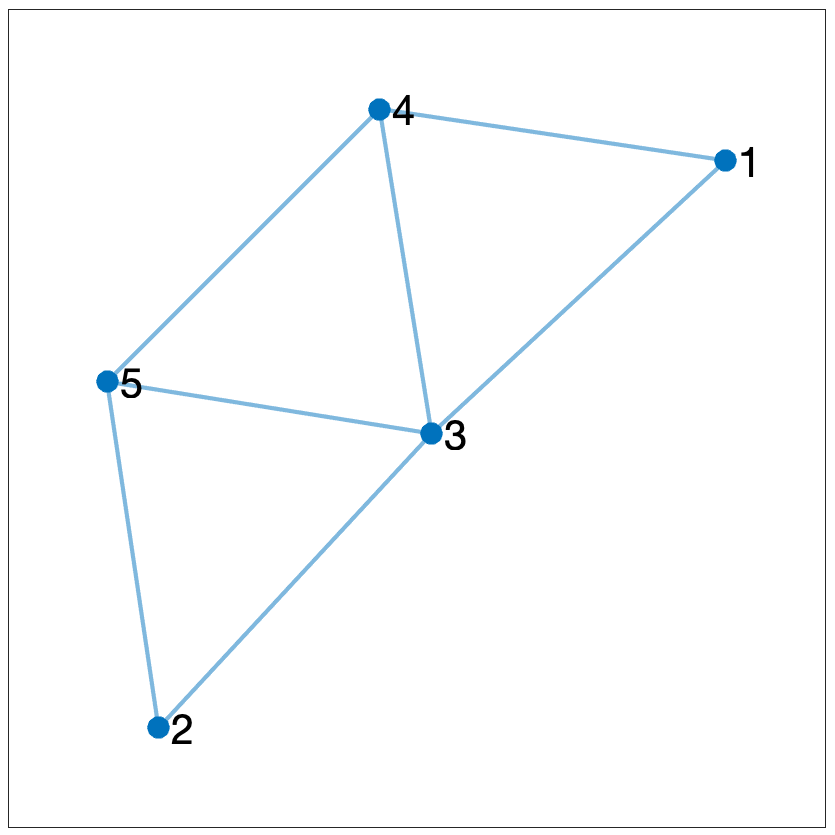
\includegraphics[width=.9\textwidth]{./img/tracking/graph1.pdf}
        \caption{无权重无向图}
        \label{fig_graph_eg_1}
    \end{subfigure}
    \begin{subfigure}{.3\textwidth}
        \centering
        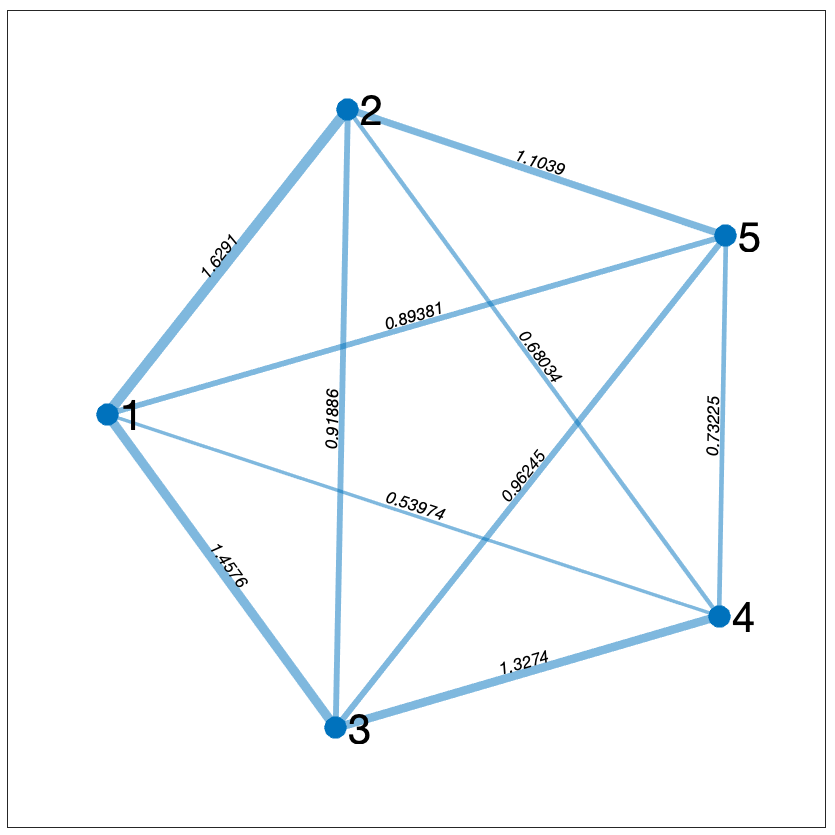
\includegraphics[width=.9\textwidth]{./img/tracking/graph2.pdf}
        \caption{有权重无向图}
        \label{fig_graph_eg_2}
    \end{subfigure}
    \caption{无向图示例}
    \label{fig_graph_eg}
\end{figure}

通常,无向图的边集合 $\mathcal E$ 可以用一个对称的矩阵 $\mathbf E \in \mathbb R^{n \times n}$ 表示,其中的元素表示节点之间的连接关系或权重。例如,\cref{fig_graph_eg} 所示的两个图,其边的集合对应的矩阵为
$$
    \mathbf{E}_1 =
    \begin{bmatrix}
        0 & 0 & 1 & 1 & 0 \\
        0 & 0 & 1 & 0 & 1 \\
        1 & 1 & 0 & 1 & 1 \\
        1 & 0 & 1 & 0 & 1 \\
        0 & 1 & 1 & 1 & 0 \\
    \end{bmatrix} \quad \mathbf{E}_2 =
    \begin{bmatrix}
        0.00 & 1.63 & 1.46 & 0.54 & 0.89 \\
        1.63 & 0.00 & 0.92 & 0.68 & 1.10 \\
        1.46 & 0.92 & 0.00 & 1.33 & 0.96 \\
        0.54 & 0.68 & 1.33 & 0.00 & 0.73 \\
        0.89 & 1.10 & 0.96 & 0.73 & 0.00 \\
    \end{bmatrix}
$$
